\section{infoarea.h File Reference}
\label{infoarea_8h}\index{infoarea.h@{infoarea.h}}


{\tt \#include $<$qwidget.h$>$}\par
{\tt \#include $<$qpixmap.h$>$}\par
{\tt \#include $<$kurl.h$>$}\par
{\tt \#include $<$qlistview.h$>$}\par
{\tt \#include $<$qvaluelist.h$>$}\par
{\tt \#include $<$qlabel.h$>$}\par
{\tt \#include \char`\"{}skinbutton.h\char`\"{}}\par
{\tt \#include \char`\"{}global\_\-define.h\char`\"{}}\par
{\tt \#include \char`\"{}hdassplaylistitem.h\char`\"{}}\par
{\tt \#include \char`\"{}hdassplaylist.h\char`\"{}}\par
{\tt \#include \char`\"{}enum.h\char`\"{}}\par


Include dependency graph for infoarea.h:\begin{figure}[H]
\begin{center}
\leavevmode
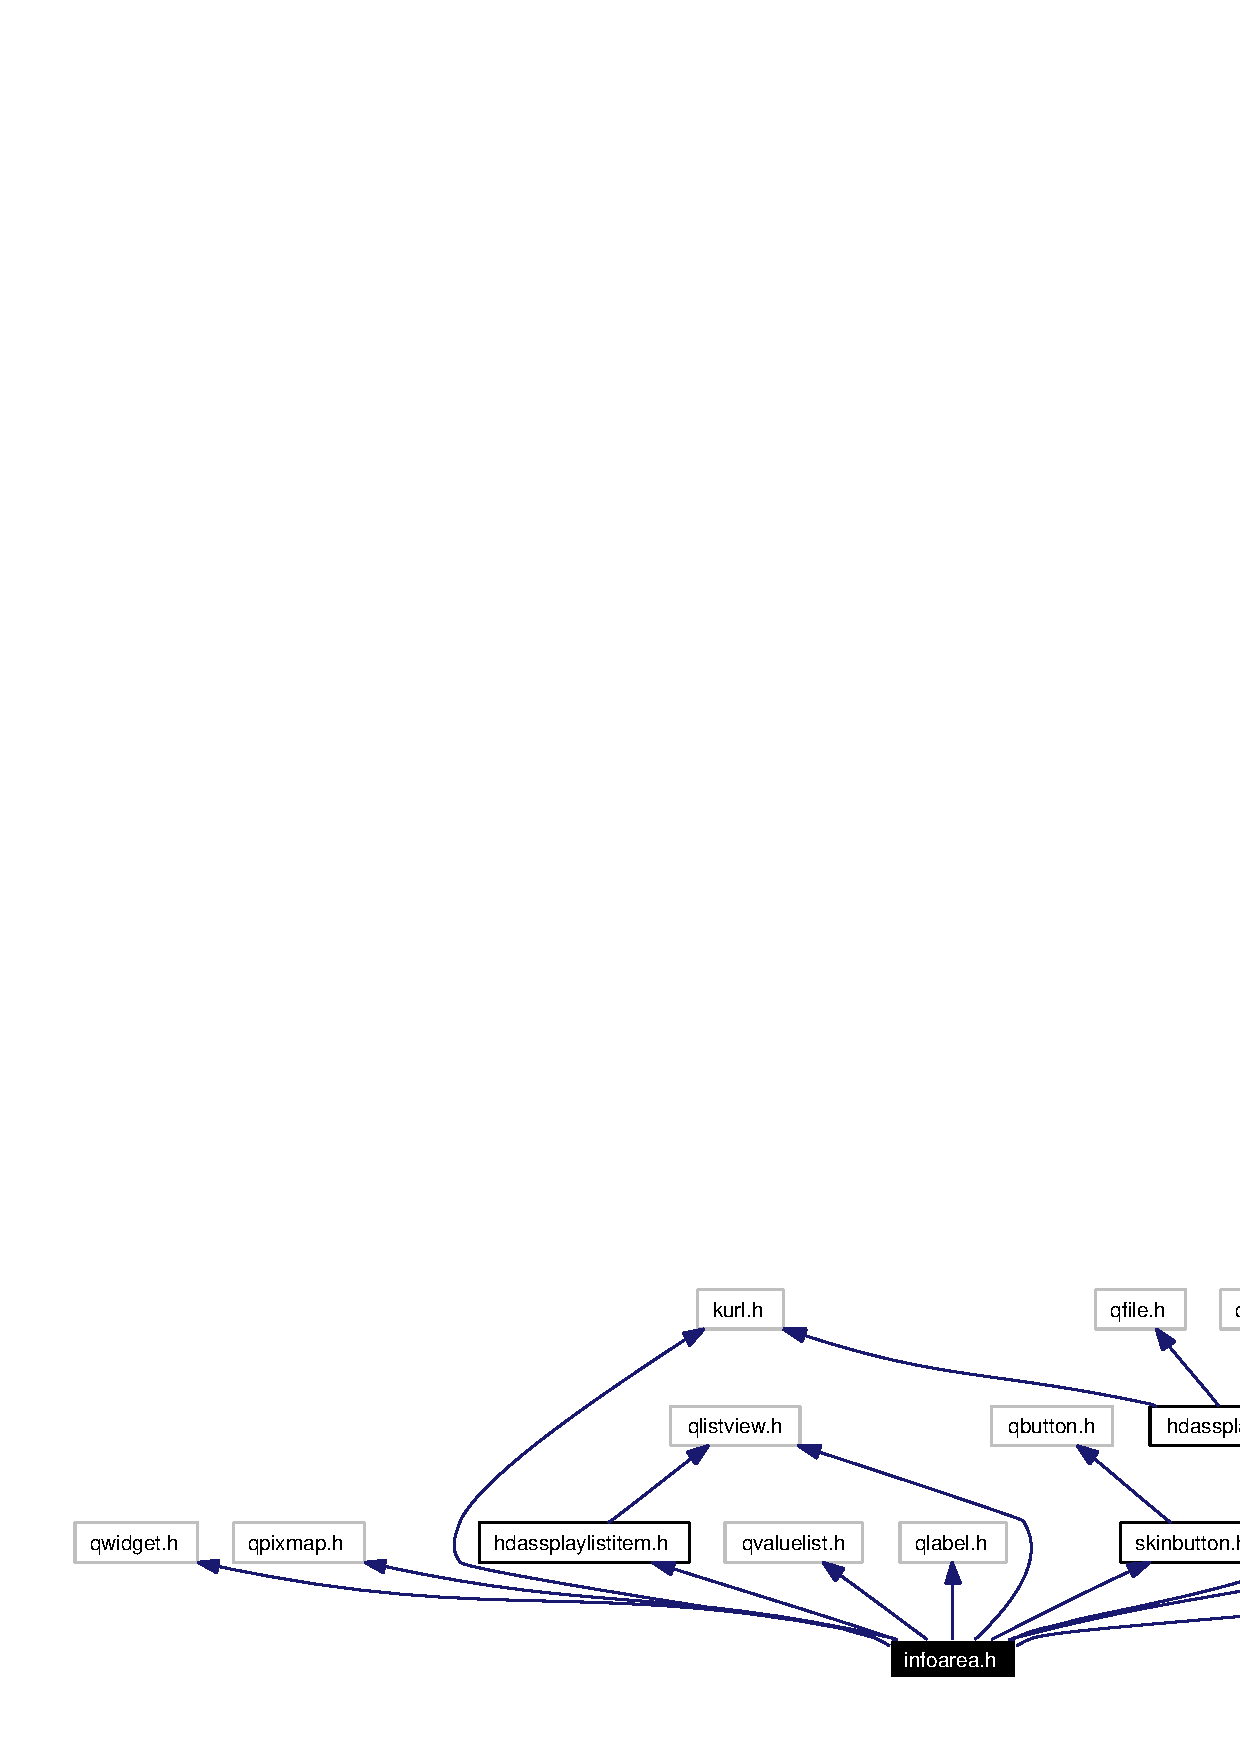
\includegraphics[width=399pt]{infoarea_8h__incl}
\end{center}
\end{figure}


This graph shows which files directly or indirectly include this file:\begin{figure}[H]
\begin{center}
\leavevmode
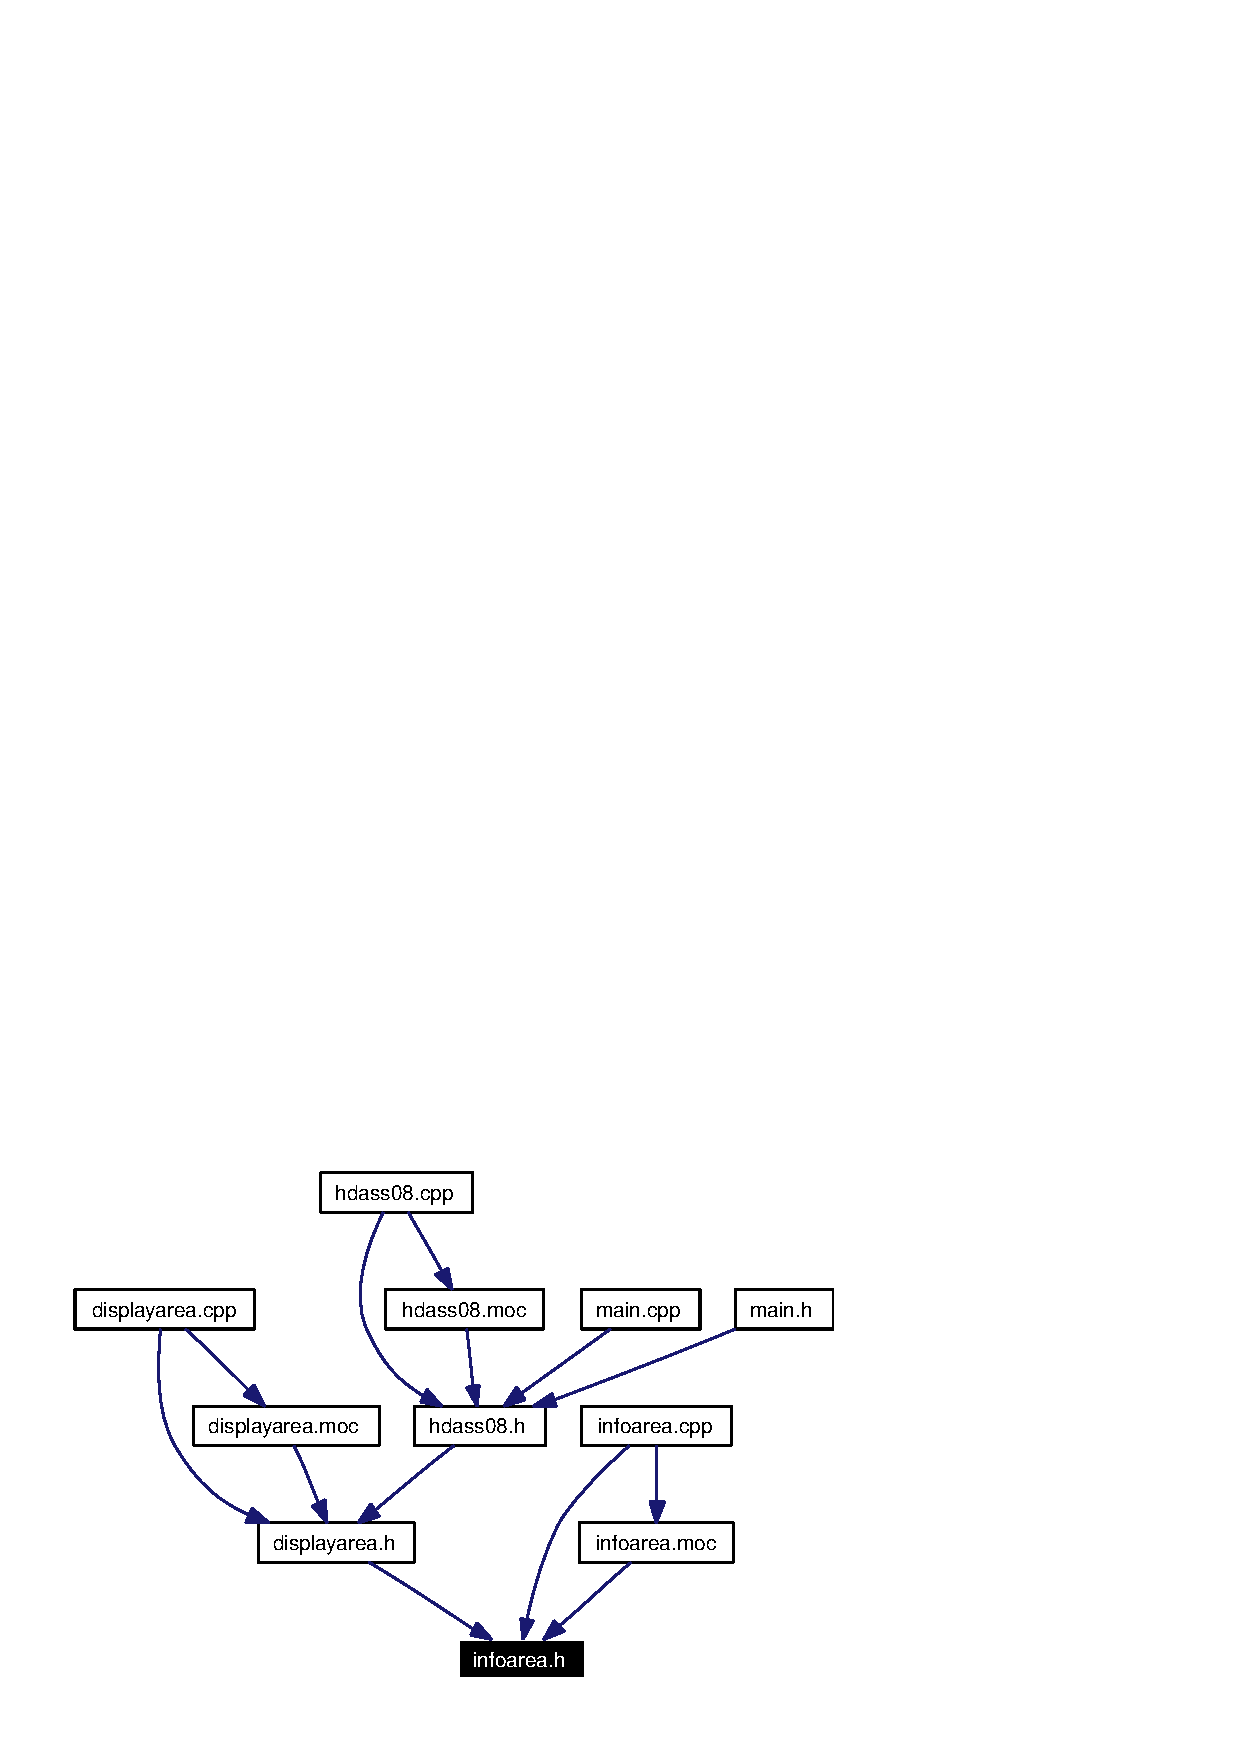
\includegraphics[width=200pt]{infoarea_8h__dep__incl}
\end{center}
\end{figure}
\subsection*{Classes}
\begin{CompactItemize}
\item 
class {\bf Info\-Area}
\end{CompactItemize}
